\section{Project Objective}

%\begin{itemize}

   % \item Briefly summarize the purpose of the analysis and its abstracts. Highlight the implications for the recommend system.
    
   % \item Provide an introduction to the report, explaining the context and goals of the hierarchical cluster analysis.
%\end{itemize}

%\begin{enumerate}
  %  \item We would like to group together users with similar viewing patterns in order to recommend similar content (genres). By asking different questions about age, genre, hobbies, we can collect data and conclude some insights.

   %  \item The data will be collect and analysis by using R software 

    
 
  
      We would like to group together users with similar viewing patterns in order to recommend similar content (genres). By asking different questions about age, genre, hobbies, we can collect data and conclude some insights.

    

    

    
   % \end{itemize}

%\end{enumerate}

\section {Overview of Hierarchical clustering methodology}
Hierarchical clustering is an algorithm that groups similar objects into clusters. The clusters are distinct from each other, and the objects within each cluster are broadly similar to each other.

Hierarchical clustering is an unsupervised learning technique. This means that a model does not have to be trained, and there is no need for a "target" variable.

There are two common categories of Hierarchical clustering, agglomerative and divisive. 

\begin{itemize}
    \item Agglomerative clustering starts in it individual clusters, then merges pair of clusters and continuing until all clusters have been merge in one huge clusters.

        \begin{figure}[H]
            \centering
            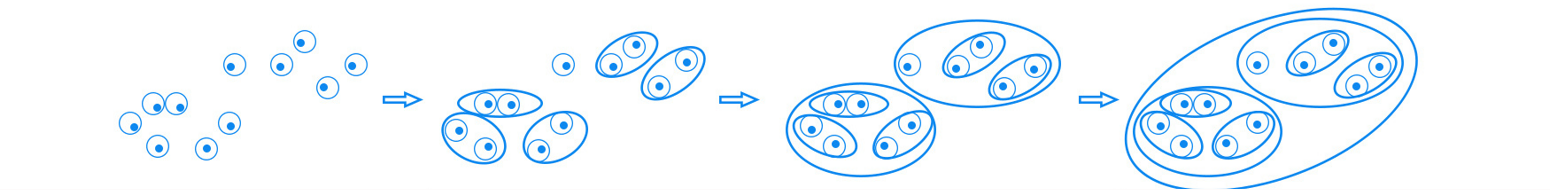
\includegraphics[scale=0.4]{graphics/overview/Agglomerative.png}
            \caption{Agglomerative clustering}
        \end{figure}

    \item Divisive clustering is the inverse approach of agglomerative clustering which starts in one cluster then splits into smaller cluster base on their difference.

        \begin{figure}[H]
            \centering
            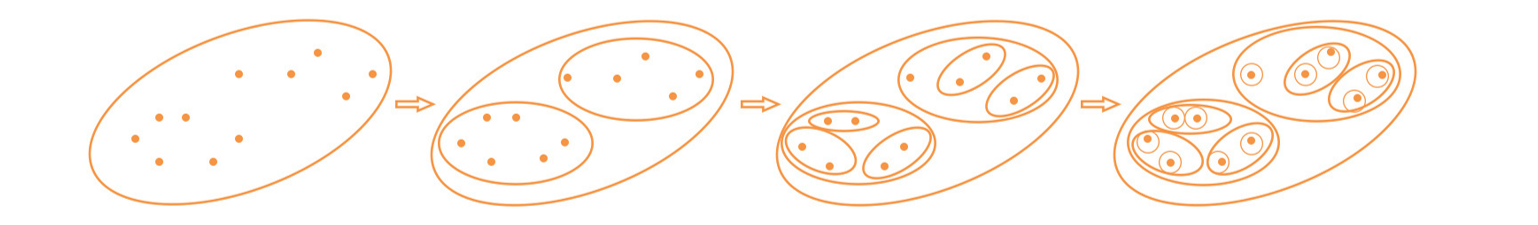
\includegraphics[scale=0.4]{graphics/overview/Diversive.png}
            \caption{Divisive clustering}
        \end{figure}
\end{itemize}
In our project, we only focus on agglomerative clustering.




The method of hierarchical clustering starts by treating each data point as a separate cluster and then iteratively combines the closest clusters until a stopping criterion is reached. The clusters are visually represented in a hierarchical tree called a dendrogram. 

\begin{figure}[H]
     \centering
     \begin{subfigure}[b]{0.3\textwidth}
         \centering
         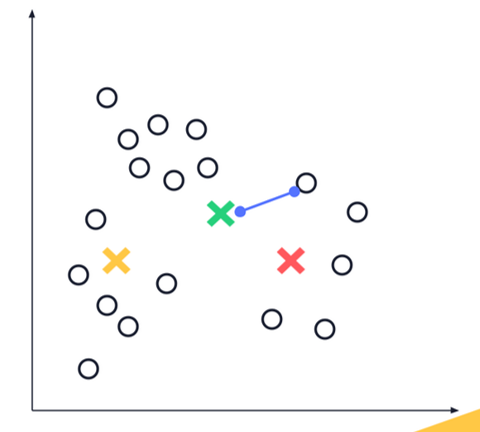
\includegraphics[width=\textwidth]{graphics/overview/FIndDistance.png}
         \caption{Finding points distances}
         % \label{fig:audau1701}
     \end{subfigure}
     \hfill
     \begin{subfigure}[b]{0.3\textwidth}
         \centering
         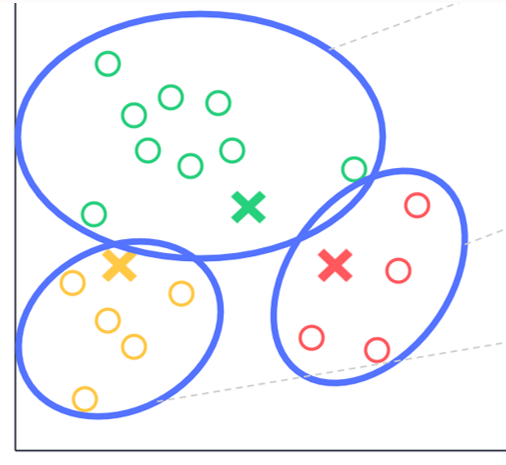
\includegraphics[width=\textwidth]{graphics/overview/Grouping.png}
         \caption{Grouping}
     \end{subfigure}
     \hfill
     \begin{subfigure}[b]{0.3\textwidth}
         \centering
         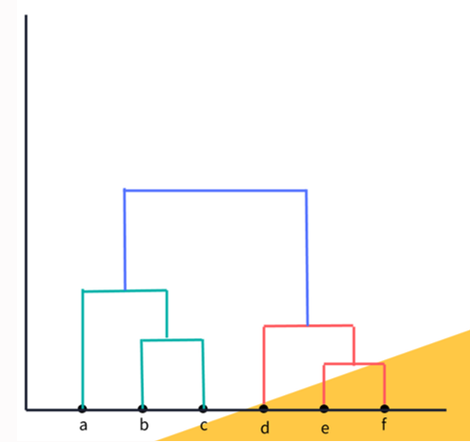
\includegraphics[width=\textwidth]{graphics/overview/Termination.png}
         \caption{Termination}
     \end{subfigure}
        \caption{Hierarchical clustering steps}
\end{figure}

\begin{enumerate}
    \item \textbf{Finding points distances:} Calculate the distance between each point of observation. There are various mathematical algorithms to apply: "euclidean", "maximum", "manhattan", "canberra", "binary", "minkowski"

    \item \textbf{Grouping points (clustering)} Calculate the distance between each cluster. There are various mathematical algorithms to apply:"Ward", "single", "complete", "average", "mcquitty", "median", "centroid". After that, choose the optimal number of clusters. 

    \item \textbf{Termination} Plotting the final dendrogram and starting the analysis process based on attributes of each cluster.
\end{enumerate}

